% EPN, Tue Jun 12 16:53:45 2012
% Actual commands run on: 
% MacBook Pro, mid 2009
% 2.53 GHz Intel Core 2 Duo
% 4 Gb 1067 MHz DDR3 (RAM)

\section{Tutorial}
\label{section:tutorial}
\setcounter{footnote}{0}

Here's a tutorial walk-through of some small projects with
Infernal. This should suffice to get you started on work of your own,
and you can (at least temporarily) skip the rest of the Guide,
such as all the nitty-gritty details of available command line
options.

\subsection {The programs in Infernal}


\begin{tabular}{ll}
\multicolumn{2}{c}{\textbf{Core programs}}\\
 & \\ 
\textbf{cmbuild}     & Build a covariance model from an input multiple alignment.\\
\textbf{cmcalibrate} & Calibrate E-value parameters for a covariance model.\\
\textbf{cmsearch}    & Search a covariance model against a sequence database.\\
\textbf{cmscan}      & Search a sequence against a covariance model database.\\
\textbf{cmalign}     & Make a multiple alignment of many sequences to a common covariance model.\\
 & \\ 
\multicolumn{2}{c}{\textbf{Other utilities}}\\ 
 & \\ 
\textbf{cmconvert} & Convert CM formats to/from Infernal v1.1 format.\\ 
\textbf{cmemit}    & Generate (sample) sequences from a covariance model.\\
\textbf{cmfetch}   & Get a covariance model by name or accession from a CM database.\\
\textbf{cmpress}   & Format a CM database into a binary format for \prog{cmscan}.\\
\textbf{cmstat}    & Show summary statistics for each model in a CM database.\\ 
\end{tabular} \\
\\

In this section, we'll show examples of running each of these
programs, using examples in the \otext{tutorial/} subdirectory of the
distribution.

\subsection{Files used in the tutorial}

The subdirectory \otext{/tutorial} in the Infernal distribution contains the
files used in the tutorial, as well as a number of examples of various
file formats that Infernal reads. The important files for the tutorial
are:

\begin{sreitems}{\emprog{minifam.i1\{m,i,f,p\}}}
\item[\otext{tRNA5.sto}] A multiple alignment of five tRNA
  sequences. This file is a simple example of \emph{Stockholm
  format} that Infernal uses for structurally-annotated alignments.
%
\item[\otext{tRNA5.c.cm}] An example CM file. Built with
  \prog{cmbuild} from \otext{tRNA5.sto} and calibrated using
  \prog{cmcalibrate}. Included so you don't need to calibrate your own
  model file, which takes about 20 minutes. 
%
\item[\otext{mrum-genome.fa}]: The 3 Mb genome of the methanogenic archeaon 
  \emph{Methanobrevibacter ruminantium}, in
  FASTA format, downloaded from the NCBI Nucleotide database
  (accession: NC\_13790.1). 
%
\item[\otext{tRNA5-mrum.out}]: An example \prog{cmsearch} output file,
  obtained by searching \otext{tRNA5.c.cm} against \otext{mrum-genome.fa}.
%
\item[\otext{5S\_rRNA.sto}]: The Rfam 10.1 5S ribosomal RNA (RF00001) 
  ``seed'' alignment. 
%
\item[\otext{5S\_rRNA.c.cm}]: A CM file built from
  \otext{5S\_rRNA.sto} using \prog{cmbuild}
  and calibrated using \prog{cmcalibrate}.
%
\item[\otext{Cobalamin.sto}]: The Rfam 10.1 Cobalamin riboswitch (RF00174) 
  ``seed'' alignment. 
%
\item[\otext{Cobalamin.c.cm}]: A CM file built from
  \otext{Cobalamin.sto} using \prog{cmbuild}
  and calibrated using \prog{cmcalibrate}.
%
\item[\otext{minifam.cm}]: A CM file including three calibrated CMs.
  This is actually just a concatenation 
  of the files \otext{tRNA5.c.cm}, \otext{5S\_rRNA.c.cm} and
  \otext{Cobalamin.c.cm}.
%
\item[\emprog{minifam.i1\{m,i,f,p\}}] Binary compressed files
  corresponding to \otext{minifam.cm}, produced by \prog{cmpress}.
%
\item[\otext{metag-example.fa}]: A FASTA sequence file containing 3
  sequences hand-selected from a metagenomics dataset \citep{Tringe05},
  used for demonstrating \prog{cmscan}. 
%
\item[\otext{minifam-metag.out}]: An example \prog{cmscan} output file,
  obtained by searching \otext{minifam.cm} against \otext{metag-example.fa}.
%
\item[\otext{mrum-tRNAs10.fa}]: A FASTA sequence file containing 10
  tRNAs predicted using \prog{cmsearch} in the \emph{M. ruminantium} genome.
%
\item[\otext{mrum-tRNAs10.out}]: An example \prog{cmalign} output
  alignment, obtained by aligning the sequences in
  \otext{mrum-tRNAs10.fa} to the model in \otext{tRNA5.c.cm} with \prog{cmalign}.
%
\item[\otext{Cobalamin.fa}]: A FASTA sequence file containing 1
  \prog{cmscan}-predicted Cobalamin riboswitch extracted from \otext{metag-example.fa}.
%
\item[\otext{tRNA5-noss.sto}]: A Stockholm alignment file identical
  to \otext{tRNA.sto} except without secondary structure annotation.
  Used to demonstrate HMM searches for models without secondary
  structure.
%
\item[\otext{tRNA5-hand.sto}]: A Stockholm alignment file identical
  to \otext{tRNA.sto} except it includes column reference annotation.
  Used to demonstrate expert annotation of model positions with
  \otext{cmbuild --hand}.
%
\item[\otext{tRNA5-hand.c.cm}]: A CM file built from
  \otext{tRNA5-hand.sto} with \prog{cmbuild} and calibrated with
  \prog{cmcalibrate}. 
\end{sreitems}

\subsection{Searching a sequence database with a single covariance model}

\subsubsection{Step 1: build a covariance model with cmbuild}

Infernal starts with a multiple sequence alignment file that you
provide. It must be in Stockholm format and must include consensus
secondary structure annotation. The file \otext{tutorial/tRNA5.sto} is
an example of a simple Stockholm file. It is shown below, with a
secondary structure of the first sequence shown to the right for
reference (yeast Phe tRNA, labeled as ``tRNA1'' in the file):

\vspace{1em}
\begin{minipage}{4.7in}
\begin{sreoutput}[xleftmargin=0em]
# STOCKHOLM 1.0

tRNA1             GCGGAUUUAGCUCAGUUGGG.AGAGCGCCAGACUGAAGAUCUGGAGGUCC
tRNA2             UCCGAUAUAGUGUAAC.GGCUAUCACAUCACGCUUUCACCGUGGAGA.CC
tRNA3             UCCGUGAUAGUUUAAU.GGUCAGAAUGGGCGCUUGUCGCGUGCCAGA.UC
tRNA4             GCUCGUAUGGCGCAGU.GGU.AGCGCAGCAGAUUGCAAAUCUGUUGGUCC
tRNA5             GGGCACAUGGCGCAGUUGGU.AGCGCGCUUCCCUUGCAAGGAAGAGGUCA
#=GC SS_cons      <<<<<<<..<<<<.........>>>>.<<<<<.......>>>>>.....<

tRNA1             UGUGUUCGAUCCACAGAAUUCGCA
tRNA2             GGGGUUCGACUCCCCGUAUCGGAG
tRNA3             GGGGUUCAAUUCCCCGUCGCGGAG
tRNA4             UUAGUUCGAUCCUGAGUGCGAGCU
tRNA5             UCGGUUCGAUUCCGGUUGCGUCCA
#=GC SS_cons      <<<<.......>>>>>>>>>>>>.
//
\end{sreoutput}
\end{minipage}
\begin{minipage}{1.5in}
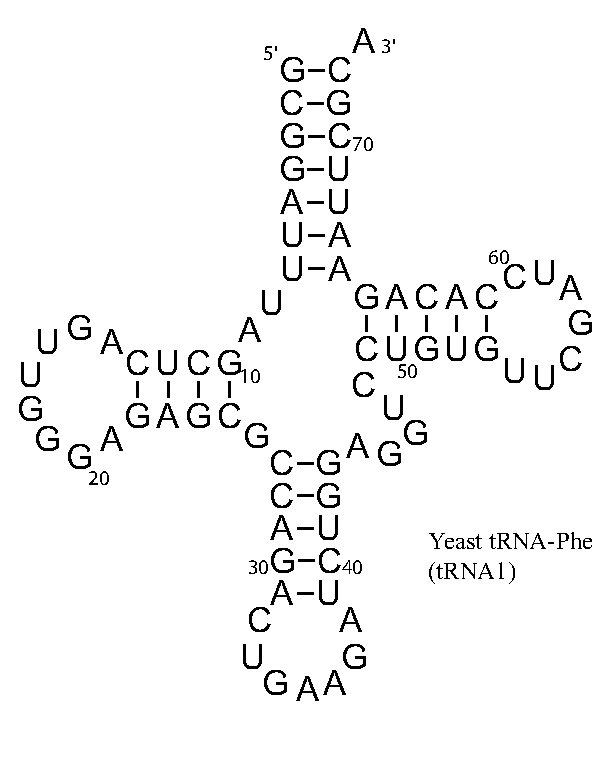
\includegraphics[scale=0.4]{Figures/trna1-DF6280}
\end{minipage}
\vspace{1em}

This is a simple example of a multiple RNA sequence alignment with
secondary structure annotation, in \emph{Stockholm format}.  Stockholm
format, the native alignment format used by HMMER and Infernal and the
Pfam and Rfam databases, is documented in detail later in the guide in
section~\ref{section:stockholm}.

For now, what you need to know about the key features of the input file is:
\begin{itemize}
\item The alignment is in an interleaved format.
Lines consist of a name, followed by an aligned sequence;
long alignments are split into blocks separated by blank lines.
\item Each sequence must have a unique name that has zero spaces in it. (This is important!)
\item For residues, any one-letter IUPAC nucleotide code is accepted,
      including ambiguous nucleotides. Case is ignored; residues
      may be either upper or lower case.
\item Gaps are indicated by the characters \otext{.}, \otext{\_}, -, or \otext{~}.
      (Blank space is not allowed.)
\item A special line starting with \otext{\#=GC SS\_cons} indicates
      the secondary structure consensus. Gap characters annotate
      unpaired (single-stranded) columns. Base pairs are indicated
      by any of the following pairs: \otext{<>}, \otext{()}, \otext{[]},
      or \otext{[]}. No pseudoknots are allowed; the
      open/close-brackets notation is only unambiguous for strictly
      nested base-pairing interactions.
      For more on secondary structure annotation see
      section~\ref{section:wuss}.
\item The alignment begins with the special tag line
      \otext{\# STOCKHOLM 1.0}, and ends with \otext{//}.
      Stockholm alignments
      can be concatenated to create an alignment database flatfile
      containing many alignments.
\end{itemize}

The \prog{cmbuild} command builds a covariance model from an alignment (or
CMs for each of many alignments in a Stockholm file), and saves the
CM(s) in a file. For example, type:

\user{cmbuild tRNA5.cm tutorial/tRNA5.sto}

and you'll see some output that looks like:

\begin{sreoutput}
# cmbuild :: covariance model construction from multiple sequence alignments
# INFERNAL 1.1 (June 2012)
# Copyright (C) 2012 Howard Hughes Medical Institute.
# Freely distributed under the GNU General Public License (GPLv3).
# - - - - - - - - - - - - - - - - - - - - - - - - - - - - - - - - - - - -
# CM file:                                            tRNA5.cm
# alignment file:                                     ../tutorial/tRNA5.sto
# - - - - - - - - - - - - - - - - - - - - - - - - - - - - - - - - - - - -
#                                                                      rel entropy
#                                                                      -----------
# idx    name                     nseq eff_nseq   alen  clen  bps bifs    CM   HMM description
# ------ -------------------- -------- -------- ------ ----- ---- ---- ----- ----- -----------
       1 tRNA5                       5     3.73     74    72   21    2 0.783 0.489 
#
# CPU time: 0.34u 0.00s 00:00:00.34 Elapsed: 00:00:00.71
\end{sreoutput}

If your input file had contained more than one alignment, you'd get
one line of output for each model. The information on these lines is
almost self-explanatory. The \otext{tRNA5} alignment consisted of 5
%  VERIFY WHEN UPDATING                                          ^
sequences with 74 aligned columns. Infernal turned it into a model of
%              ^^
72 consensus positions, which means it defined 2 gap-containing
%^                                             ^
alignment columns to be insertions relative to consensus. The 5
%                                                             ^
sequences were only counted as an ``effective'' total sequence number
(\otext{eff\_nseq}) of 3.73. The model includes 21 basepairs and 2
%                     ^^^^                     ^^               ^
bifurcations. The model ended up with a relative entropy per position
(\otext{rel entropy, CM}; information content) of 0.783 bits. If the
%                                                ^^^^^
secondary structure information of the model were ignored the relative
entropy per position (\otext{rel entropy, HMM}) would be 0.489 bits.
%                                                       ^^^^^         
This output format is rudimentary. Infernal knows quite a bit more
information about what it's done to build this CM, but it's not
displaying it. You don't need to know more to be able to use the
model, so we can press on here. Model construction is described in
more detail in section~\ref{section:cmbuild}.

The new CM was saved to \otext{tRNA5.cm}. You can look at it
(e.g. \otext{> more tRNA5.cm}) if you like, but it isn't really designed
to be human-interpretable. You can treat \otext{.cm} files as compiled
models of your RNA alignment. The Infernal ASCII save file format is
defined in Section~\ref{section:formats}.

\subsubsection{Step 2: calibrate the model with cmcalibrate}

The next step is to ``calibrate'' the model. This step must be
performed priot to using your model for database searches with
\prog{cmsearch} or \prog{cmscan}. In this step, statistical parameters
necessary for reporting E-values (expectation values) are estimated
and stored in the CM file. When \prog{cmsearch} or \prog{cmscan} is
later used for a database search and a hit with score $x$ is found,
the E-value of that hit is the number of hits expected to score $x$ or
more just by chance (given the size of the search you're performing).

\emph{Importantly, if you're not going to use a model for database
search, there is no need to calibrate it.} For example, if you are
only going to use a model to create structurally annotated multiple
alignments of a large family like small subunit ribosomal RNA, don't
waste time calibrating it. \prog{cmsearch} and \prog{cmscan} are the
only Infernal programs that use E-values, so if you're not going to
use them then don't calibrate your model.

Unfortunately, CM calibration takes a long time because fairly long
random sequences must be searched to determine the expected
distribution of hit scores against nonhomologous sequences, and none
of the search acceleration heuristics described in
section~\ref{section:pipeline} can be used because they rely on
detecting primary sequence similarity which is absent in random
sequence. 

The amount of time required for calibration varies widely, but
depends mainly on the size of the RNA family being modeled.
So you can know what kind of a wait you're in for, the
\prog{cmcalibrate} has a \otext{--forecast} option which reports an
estimate of the running time. To get an estimate for the tRNA model, do:

\user{cmcalibrate --forecast tRNA5.cm}\\

You should see something like this:

\begin{sreoutput}
<[src]> ./cmcalibrate --forecast tRNA5.cm
# cmcalibrate :: fit exponential tails for CM E-values
# INFERNAL 1.1 (June 2012)
# Copyright (C) 2012 Howard Hughes Medical Institute.
# Freely distributed under the GNU General Public License (GPLv3).
# - - - - - - - - - - - - - - - - - - - - - - - - - - - - - - - - - - - -
# CM file:                                     tRNA5.cm
# forecast mode (no calibration):              on (2 CPUs)
# - - - - - - - - - - - - - - - - - - - - - - - - - - - - - - - - - - - -
#
# Forecasting running time for CM calibration(s) on 2 cpus:
#
#                          predicted
#                       running time
# model name            (hr:min:sec)
# --------------------  ------------
  tRNA5                     00:20:37
#
# CPU time: 0.22u 0.01s 00:00:00.23 Elapsed: 00:00:00.30
[ok]
\end{sreoutput}

The header comes first, telling you what program you ran, on what file
and with what options. This calibration will use 2 CPUs, your output
may vary depending on how many cores you have available on the machine
you're using\footnote{All the exercises in this tutorial were
  performed on a mid 2009 MacBook Pro with 2 cores}. (If you are
planning to use MPI to parallelize the calibration (see the
Installation section), you can specify the number of CPUs for the time
estimate as \otext{<n>} with the \otext{--nforecast <n>} option.) Using
2 CPUs, \prog{cmcalibrate} estimates the time required for calibration
on the machine I'm using at about twenty minutes.

Feel free to perform the calibration yourself if you'd like (with the
command \otext{cmcalibrate tRNA5.cm}). However, we've included the file
\otext{tRNA5.c.cm}, an already calibrated version of \otext{tRNA5.cm},
for you to use if you don't want to wait. To use this calibrated
model, copy over the \otext{tRNA5.cm} file you just made with the
calibrated version:
 
\user{cp tRNA5.c.cm tRNA5.cm}\\
 
\subsubsection{Step 3: search a sequence database with cmsearch}

You can now use your tRNA model to search for tRNA homologs in a
database. The file \otext{mrum-genome.fa} is the genome sequence of the
archaeon \emph{Methanobrevibacter rumanitium} (accession:
\otext{NC\_13790.1}). We'll use this file as our database. To perform
the search:

\user{cmsearch tRNA5.cm mrum-genome.fa}\\

As before, the first section is the header, telling you what program
your ran, on what, and with what options, as well as the name and size
of:

\begin{sreoutput}
# cmsearch :: search CM(s) against a sequence database
# INFERNAL 1.1 (June 2012)
# Copyright (C) 2012 Howard Hughes Medical Institute.
# Freely distributed under the GNU General Public License (GPLv3).
# - - - - - - - - - - - - - - - - - - - - - - - - - - - - - - - - - - - -
# query CM file:                         tRNA5.cm
# target sequence database:              ../tutorial/mrum-genome.fa
# number of worker threads:              2
# - - - - - - - - - - - - - - - - - - - - - - - - - - - - - - - - - - - -
\end{sreoutput}

The second section is a list of ranked top hits (sorted by E-value,
most significant hit first):

% tutorial regression: tRNA5-search.out
\begin{sreoutput}
 rank     E-value  score  bias  sequence      start     end   mdl trunc   gc  description
 ----   --------- ------ -----  ----------- ------- -------   --- ----- ----  -----------
  (1) !   1.3e-18   71.5   0.0  NC_013790.1  362026  361955 -  cm    no 0.50  Methanobrevibacter ruminantium M1 chromosome, complete genome
  (2) !   3.3e-18   70.2   0.0  NC_013790.1 2585265 2585193 -  cm    no 0.60  Methanobrevibacter ruminantium M1 chromosome, complete genome
  (3) !     9e-18   68.8   0.0  NC_013790.1  762490  762562 +  cm    no 0.67  Methanobrevibacter ruminantium M1 chromosome, complete genome
  (4) !     9e-18   68.8   0.0  NC_013790.1 2041704 2041632 -  cm    no 0.67  Methanobrevibacter ruminantium M1 chromosome, complete genome
  (5) !   2.5e-17   67.4   0.0  NC_013790.1 2351254 2351181 -  cm    no 0.62  Methanobrevibacter ruminantium M1 chromosome, complete genome
  (6) !     3e-17   67.2   0.0  NC_013790.1  735136  735208 +  cm    no 0.59  Methanobrevibacter ruminantium M1 chromosome, complete genome
  (7) !   5.2e-17   66.4   0.0  NC_013790.1 2186013 2185941 -  cm    no 0.53  Methanobrevibacter ruminantium M1 chromosome, complete genome
  (8) !   1.6e-16   64.8   0.0  NC_013790.1 2350593 2350520 -  cm    no 0.66  Methanobrevibacter ruminantium M1 chromosome, complete genome
  (9) !   2.8e-16   64.1   0.0  NC_013790.1 2585187 2585114 -  cm    no 0.59  Methanobrevibacter ruminantium M1 chromosome, complete genome
 (10) !   9.1e-16   62.5   0.0  NC_013790.1  662185  662259 +  cm    no 0.61  Methanobrevibacter ruminantium M1 chromosome, complete genome
 (11) !   1.2e-15   62.1   0.0  NC_013790.1  360887  360815 -  cm    no 0.55  Methanobrevibacter ruminantium M1 chromosome, complete genome
 (12) !   1.6e-15   61.7   0.0  NC_013790.1 2350984 2350911 -  cm    no 0.53  Methanobrevibacter ruminantium M1 chromosome, complete genome
 (13) !   3.3e-15   60.7   0.0  NC_013790.1 2186090 2186019 -  cm    no 0.54  Methanobrevibacter ruminantium M1 chromosome, complete genome
 (14) !   4.1e-15   60.4   0.0  NC_013790.1 2680159 2680233 +  cm    no 0.67  Methanobrevibacter ruminantium M1 chromosome, complete genome
 (15) !   7.9e-15   59.5   0.0  NC_013790.1 2749839 2749768 -  cm    no 0.53  Methanobrevibacter ruminantium M1 chromosome, complete genome
 (16) !   7.9e-15   59.5   0.0  NC_013790.1 2749945 2749874 -  cm    no 0.53  Methanobrevibacter ruminantium M1 chromosome, complete genome
 (17) !   9.8e-15   59.2   0.0  NC_013790.1  361676  361604 -  cm    no 0.51  Methanobrevibacter ruminantium M1 chromosome, complete genome
 (18) !     1e-14   59.2   0.0  NC_013790.1 2585073 2584999 -  cm    no 0.60  Methanobrevibacter ruminantium M1 chromosome, complete genome
 (19) !   1.1e-14   59.1   0.0  NC_013790.1 2130422 2130349 -  cm    no 0.59  Methanobrevibacter ruminantium M1 chromosome, complete genome
 (20) !   1.2e-14   58.9   0.0  NC_013790.1  546056  545947 -  cm    no 0.61  Methanobrevibacter ruminantium M1 chromosome, complete genome
 (21) !   3.9e-14   57.3   0.0  NC_013790.1  361915  361844 -  cm    no 0.42  Methanobrevibacter ruminantium M1 chromosome, complete genome
 (22) !   5.1e-14   57.0   0.0  NC_013790.1   97724   97795 +  cm    no 0.49  Methanobrevibacter ruminantium M1 chromosome, complete genome
 (23) !   6.1e-14   56.7   0.0  NC_013790.1 2350717 2350646 -  cm    no 0.68  Methanobrevibacter ruminantium M1 chromosome, complete genome
 (24) !     8e-14   56.3   0.0  NC_013790.1 1873887 1873815 -  cm    no 0.64  Methanobrevibacter ruminantium M1 chromosome, complete genome
 (25) !   1.4e-13   55.6   0.0  NC_013790.1  360730  360659 -  cm    no 0.40  Methanobrevibacter ruminantium M1 chromosome, complete genome
 (26) !   3.5e-13   54.3   0.0  NC_013790.1 2680310 2680384 +  cm    no 0.52  Methanobrevibacter ruminantium M1 chromosome, complete genome
 (27) !   3.6e-13   54.3   0.0  NC_013790.1 2664806 2664732 -  cm    no 0.60  Methanobrevibacter ruminantium M1 chromosome, complete genome
 (28) !   3.6e-13   54.3   0.0  NC_013790.1  361061  360989 -  cm    no 0.41  Methanobrevibacter ruminantium M1 chromosome, complete genome
 (29) !   7.5e-13   53.3   0.0  NC_013790.1 2130335 2130262 -  cm    no 0.55  Methanobrevibacter ruminantium M1 chromosome, complete genome
 (30) !   7.6e-13   53.3   0.0  NC_013790.1 2151672 2151745 +  cm    no 0.65  Methanobrevibacter ruminantium M1 chromosome, complete genome
 (31) !   2.9e-12   51.4   0.0  NC_013790.1  319297  319370 +  cm    no 0.62  Methanobrevibacter ruminantium M1 chromosome, complete genome
 (32) !   3.7e-12   51.1   0.0  NC_013790.1  361753  361679 -  cm    no 0.55  Methanobrevibacter ruminantium M1 chromosome, complete genome
 (33) !   3.8e-12   51.1   0.0  NC_013790.1  360983  360912 -  cm    no 0.50  Methanobrevibacter ruminantium M1 chromosome, complete genome
 (34) !   5.9e-12   50.5   0.0  NC_013790.1  361456  361383 -  cm    no 0.50  Methanobrevibacter ruminantium M1 chromosome, complete genome
 (35) !   7.4e-12   50.1   0.0  NC_013790.1  362798  362727 -  cm    no 0.51  Methanobrevibacter ruminantium M1 chromosome, complete genome
 (36) !   8.7e-12   49.9   0.0  NC_013790.1  917722  917793 +  cm    no 0.61  Methanobrevibacter ruminantium M1 chromosome, complete genome
 (37) !   1.1e-11   49.7   0.0  NC_013790.1 2583869 2583798 -  cm    no 0.51  Methanobrevibacter ruminantium M1 chromosome, complete genome
 (38) !   1.3e-11   49.4   0.0  NC_013790.1  362324  362252 -  cm    no 0.51  Methanobrevibacter ruminantium M1 chromosome, complete genome
 (39) !   1.3e-11   49.3   0.0  NC_013790.1  360811  360740 -  cm    no 0.42  Methanobrevibacter ruminantium M1 chromosome, complete genome
 (40) !   4.3e-11   47.7   0.0  NC_013790.1 1160526 1160609 +  cm    no 0.60  Methanobrevibacter ruminantium M1 chromosome, complete genome
 (41) !   9.8e-11   46.6   0.0  NC_013790.1  362403  362331 -  cm    no 0.49  Methanobrevibacter ruminantium M1 chromosome, complete genome
 (42) !   1.1e-10   46.5   0.0  NC_013790.1 2327124 2327042 -  cm    no 0.63  Methanobrevibacter ruminantium M1 chromosome, complete genome
 (43) !   1.2e-10   46.4   0.0  NC_013790.1  995344  995263 -  cm    no 0.49  Methanobrevibacter ruminantium M1 chromosome, complete genome
 (44) !   2.3e-10   45.5   0.0  NC_013790.1  256772  256696 -  cm    no 0.57  Methanobrevibacter ruminantium M1 chromosome, complete genome
 (45) !   2.5e-10   45.3   0.0  NC_013790.1 2584830 2584758 -  cm    no 0.64  Methanobrevibacter ruminantium M1 chromosome, complete genome
 (46) !   6.1e-10   44.1   0.0  NC_013790.1 2351071 2350997 -  cm    no 0.59  Methanobrevibacter ruminantium M1 chromosome, complete genome
 (47) !   6.5e-10   44.0   0.0  NC_013790.1  362552  362482 -  cm    no 0.55  Methanobrevibacter ruminantium M1 chromosome, complete genome
 (48) !   5.2e-09   41.2   0.0  NC_013790.1 1064775 1064858 +  cm    no 0.63  Methanobrevibacter ruminantium M1 chromosome, complete genome
 (49) !   1.2e-08   40.0   0.0  NC_013790.1  361222  361150 -  cm    no 0.45  Methanobrevibacter ruminantium M1 chromosome, complete genome
 (50) !   1.2e-08   40.0   0.0  NC_013790.1  361369  361297 -  cm    no 0.60  Methanobrevibacter ruminantium M1 chromosome, complete genome
 (51) !   4.8e-08   38.1   0.0  NC_013790.1  361596  361513 -  cm    no 0.61  Methanobrevibacter ruminantium M1 chromosome, complete genome
 (52) !   3.2e-07   35.5   0.0  NC_013790.1 1913310 1913227 -  cm    no 0.64  Methanobrevibacter ruminantium M1 chromosome, complete genome
 (53) !   2.6e-06   32.7   0.0  NC_013790.1  363464  363381 -  cm    no 0.51  Methanobrevibacter ruminantium M1 chromosome, complete genome
 (54) !     3e-06   32.5   0.0  NC_013790.1 2584954 2584872 -  cm    no 0.58  Methanobrevibacter ruminantium M1 chromosome, complete genome
 ------ inclusion threshold ------
 (55) ?     0.027   20.0   0.0  NC_013790.1  363803  363716 -  cm    no 0.50  Methanobrevibacter ruminantium M1 chromosome, complete genome
 (56) ?       3.4   13.4   0.0  NC_013790.1  984373  984304 -  cm    no 0.53  Methanobrevibacter ruminantium M1 chromosome, complete genome
\end{sreoutput}

The first number is the rank of each hit\footnote{Ranks of hits are in
  parantheses to make it easy to jump to/from an entry in the hit list
  and the hit alignment section, described later}. Next comes either a
\otext{!} or \otext{?} symbol and then the \emph{E-value} of the hit.
The E-value is the statistical significance of the hit: the number of
hits we'd expect to score this highly in a database of this size
(measured by the total number of nucleotides) if the database
contained only nonhomologous random sequences. The lower the E-value,
the more significant the hit. The \otext{!} or \otext{?} that
precedes the E-value indicates whether the hit does (\otext{!}) or
does not (\otext{?}) satisfy the inclusion threshold for the search.
Inclusion thresholds are used to determine what matches should be
considered to be ``true'', as opposed to reporting thresholds that
determine what matches will be reported (often including the top of
the noise, so you can see what interesting sequences might be getting
tickled by your search). By default, inclusion thresholds usually
require an E-value of 0.01 or less, and reporting E-value thresholds
are set to 10.0, but these can be changed (see the manual page for
\prog{cmsearch} in section~\ref{section:manpages}).

The E-value is based on the \emph{bit score}, which is in the next
column. This is the log-odds score for the hit. Some people like to
see a bit score instead of an E-value, because the bit score doesn't
depend on the size of the sequence database, only on the covariance
model and the target sequence.

The next number, the \emph{bias}, is a correction term for biased
sequence composition that has been applied to the sequence bit
score. Infernal uses an alternative null model we call \emph{null3},
described more in section~\ref{section:null3}, to determine the bias
bit score correction. The bias correction is often very small and is
only reported to one decimal place, after rounding. For all hits in
this example search the bias column reads 0.0 bits, indicating that
the correction is less than 0.05 bits. On very biased sequences this
correction can become significant and is helpful for lowering the
score of high-scoring false positives that achieve high scores solely
due to their biased composition. 

Next comes the target sequence name the hit is in, and the start and
end positions of the hit within the sequence. Hits can occur on either
the top (Watson) or bottom (Crick) strand of the target
sequence\footnote{You can search either only the top strand with the
\otext{--toponly} or bottom strand with the \otext{--bottomonly} options
to \prog{cmsearch} and \prog{cmscan}.}, so the start position may be
less than (if hit is on the top strand) or greater than (if hit is on
the reverse strand) the end position. After the end position, comes a single
\otext{+} or \otext{-} symbol, indicating whether the hit is on the
top (\otext{+}) or bottom (\otext{-}) strand (solely for convenience -
so you don't have to look at the start and end positions to determine
the strand the hit is on).

After the strand symbol comes the model field, which indicates whether
the hit was found using either the CM (\otext{cm}) or a profile HMM
built from the CM (\otext{hmm}). This field is necessary because for
models with zero basepairs, \prog{cmsearch} (and \prog{cmscan}) use a
profile HMM instead of a CM for final hit scoring. This is done for
reasons of speed and efficiency, because profile HMM algorithms are
more efficient than CM ones and a CM with zero basepairs is
essentially equivalent to a profile HMM. In this example, since our
tRNA model does include basepairs, \prog{cmsearch} used a CM to score
all hits and so all hits have \prog{cm} for this column. There's an
example later in the tutorial of hits found with a profile HMM.

The next column indicates whether the hit is \emph{truncated} or
not. Infernal uses special versions of its CM dynamic programming
algorithms to allow detection of structural RNAs that have been
truncated due to missing data at the beginning and/or end of a target
sequence. Truncated hits are most common in databases that include
single reads from shotgun sequencing projects. Since our database is a
complete genome, we don't expect any hits to be truncated due to
missing data. For all hits the``trunc'' column reads
``no'' indicating that, as expected, none of the hits are
truncated. There are examples of truncated hits in the next exercise
which uses \prog{cmscan}. Section~\ref{section:pipeline} describes how
Infernal detects and aligns truncated hits in more detail.

The next column reports the GC fraction of the hit. This is the
fraction of residues in the target sequence hit that are either
\otext{G} or \otext{C} residues. The GC fraction is included as an
additional indication of the level of sequence bias of the hit. Some
expert users may be aided by this number when deciding if they 
believe a hit is a real homolog or a false positive.

Finally comes the description of the sequence, if any. This
description is propogated from the input target sequence file.

After the hit list comes the hit alignments section. Each hit in 
the hit list will have a corresponding entry in this section, in the
same order. As an illustrative example, let's take a look at
hit number 43. First, take a look at the first four lines for this
hit: 

% tutorial regression: tRNA5-search.out
\begin{sreoutput}
>> NC_013790.1  Methanobrevibacter ruminantium M1 chromosome, complete genome
 rank     E-value  score  bias mdl mdl from   mdl to       seq from      seq to       acc trunc   gc
 ----   --------- ------ ----- --- -------- --------    ----------- -----------      ---- ----- ----
 (43) !   1.2e-10   46.4   0.0  cm        1       72 []      995344      995263 - .. 0.93    no 0.49
\end{sreoutput}

The first line of each hit alignment begins with \otext{>>} followed
by a single space, the name of the target sequence, then two spaces
and the description of the sequence, if any. Next comes a set of
tabular fields that is partially redundant with the information in the
hit list. The first five columns are the same as in the hit list. The
next column reports the type of model used for the alignment, as
described above for the hit list. The next four columns report the
boundaries of the alignment with respect to the query model (``mdl
from'' and ``mdl to'') and the target sequence (``seq from'' and ``seq
to''). Following the ``seq to'' column is a \otext{+} or \otext{-}
symbol indicating whether the hit is on the top (\otext{+}) or bottom
(\otext{-}) strand.

It's not immediately easy to tell from the ``to'' coordinate whether
the alignment ended internally in the query model or target sequence,
versus ran all the way (as in a full-length global alignment) to the
end(s). To make this more readily apparent, with each pair of query
and target endpoint coordinates, there's also a little symbology. For
the normal case of a non-truncated hit: \otext{..} means both ends of
the alignment ended internally, and \otext{[]} means both ends of the
alignment were full-length flush to the ends of the query or target,
and \otext{[.}  and \otext{.]} mean only the left (5') or right (3') end
was flush/full length. For truncated hits, the symbols are the same
except that either the first and/or the second symbol will be a
\otext{~} for the query and target. If the first symbol is \otext{~}
then the left end of the alignment is truncated because the 5' end of
the hit is predicted to be missing (extend beyond the beginning of the
target sequence). Similarly, if the second symbol is \otext{~} then the
right end of the alignment is truncated because the 3' end of the hit
is predicted to be missing (extend beyond the end of the target
sequence). These two symbols occur just after the ``mdl to'' column for
the query, and after the strand \otext{+} or \otext{-} symbol for the
target sequence.

The next column is labeled ``acc'' and is the average posterior
probability of the aligned target sequence residues; effectively, the
expected accuracy per residue of the alignment.

The final two columns indicate whether the hit is truncated or not and
the GC fraction of the hit. These are redundant with the columns of
the same name in the hit list, described above.

Next comes the alignment display. This is an ``optimal
posterior accuracy'' alignment \citep{Holmes98}, which means it is the
alignment with the maximal summed posterior probability of all
aligned residues. Take a look at the alignment for hit number 43:

% tutorial regression: tRNA5-search.out
\begin{sreoutput}

                                 v         v                                                            NC
                     (((((((,,<<<<______.._>>>>,<<<<<_______>>>>>,,,........,,<<<<<_______>>>>>))))))): CS
        tRNA5      1 gCcggcAUAGcgcAgUGGu..AgcgCgccagccUgucAagcuggAGg........UCCgggGUUCGAUUCcccGUgccgGca 72    
                     :::G:CAUAGCG AG GGU  A CGCG:CAG:CU +++A:CUG: G+        UC:GGGGUUCGA UCCCC:UG:C:::A
  NC_013790.1 995344 AGAGACAUAGCGAAGCGGUcaAACGCGGCAGACUCAAGAUCUGUUGAuuaguucuUCAGGGGUUCGAAUCCCCUUGUCUCUA 995263
                     **********************************************9444444445************************** PP
\end{sreoutput}

The alignment contains six lines. Start by looking at the second line
which ends with \otext{CS}.  The line shows the predicted secondary
structure of the target sequence. The format is a little fancier and
more informative than the simple least-common-denominator format we
used in the input alignment file. It's designed to make it easier to
see the secondary structure by eye. The format is described in detail
later (section~\ref{section:wuss}; for now, here's all you need to
know. Basepairs in simple stem loops are annotated with \otext{<>}
characters. Basepairs enclosing multifurcations (multiple stem loops)
are annotated with \otext{()}, such as the tRNA acceptor stem in this
example. In more complicated structures, \otext{[]} and \otext{\{\}}
annotations also show up, to reflect deeper nestings of
multifurcations. For single stranded residues, \otext{\_} characters
mark hairpin loops; \otext{-} characters mark interior loops and
bulges; \otext{,} characters mark single-stranded residues in
multifurcation loops; and \otext{:} characters mark single stranded
residues external to any secondary structure. Insertions relative to
this consensus are annotated by a \otext{.} character.

The line above the \otext{CS} line ends with \otext{NC} and marks
negative scoring non-canonical basepairs in the alignment with a
\otext{v} character. All other positions of the alignment will be
blank\footnote{For anyone trying to parse this output, this means it
is possible for this line to be completely blank except for the
\otext{NC} trailer.} More specifically, the following ten types of
basepairs which are assigned a negative score by the model at their
alignment positions will be marked with a \otext{v}: \otext{A:A},
\otext{A:C}, \otext{A:G}, \otext{C:A}, \otext{C:C}, \otext{C:U},
\otext{G:A}, \otext{G:G}, \otext{U:U}, and \otext{U:C}. The \otext{NC}
annotation makes it easy to quickly identify suspicious basepairs in
a hit. Importantly, the \otext{NC} annotation will only be present in
CM hit alignments (``mdl'' column reads ``cm'') and will be absent in
HMM hit alignments (``mdl'' column reads ``hmm'') because basepairs
are not scored by an HMM.

The third line shows that consensus of the query model. The highest
scoring residue sequence is shown. Upper case residues are highly
conserved. Lower case residues are weakly conserved or unconserved.
Dots (\otext{.}) in this line indicate insertions in the target
sequence with respect to the model.

The fourth line shows where the alignment score is coming from. For a
consensus basepair, if the observed pair is the highest-scoring
possible pair according to the consensus, both residues are shown in
upper case; if a pair has a score of $\geq 0$, both residues are
annotated by : characters (indicating an acceptable compensatory
basepair); else, there is a space, indicating that a negative
contribution of this pair to the alignment score. Note that the 
\otext{NC} line will only mark a subset of these negative scoring
pairs with a \otext{v}, as discussed above.
For a single-stranded consensus residue, if the observed residue is
the highest scoring possibility, the residue is shown in upper case;
if the observed residue has a score of $\geq 0$, a \otext{+} character
is shown; else there is a space, indicating a negative contribution to
the alignment score. Importantly for HMM hits (``mdl'' column reads
``hmm''), \emph{all} positions are considered single stranded, since
an HMM does scores each half of a basepair independently.

The fifth line, beginning with \otext{gi|288559258|ref|NC\_013790.1} is
the target sequence. Dashes (\otext{-}) in this line indicate deletions
in the target sequence with respect to the model.

The bottom line is new to version 1.1 of Infernal. This represents the
posterior probability (essentially the expected accuracy) of each
aligned residue. A 0 means 0-5\%, 1 means 5-15\%, and so on; 9 means
85-95\%, and a \otext{*} means 95-100\% posterior probability. You can
use these posterior probabilities to decide which parts of the
alignment are well-determined or not. You'll often observe, for
example, that expected alignment accuracy degrades around locations of
insertion and deletion, which you'd intuitively expect.

Alignments for some searches may be formatted slightly differently
than this example. Longer alignments to longer models will be broken
up into blocks of six lines each - this alignment was short enough to
be entirely contained within a single block.  If your model was built
with the \otext{--hand} option in \prog{cmbuild}, then an additional
line will be included in each block, with RF annotation.  If the model
used for the alignment was an HMM (the ``mdl'' column reads ``hmm'')
then the \otext{NC} line will be absent from each alignment
block. We'll see example of all three of these cases later in the
tutorial.

After hit number 43, there's 13 more hit alignments for hits number 44
through 56. 

Finally, at the bottom of the file, you'll see some summary
statistics. For example, at the bottom of the tRNA search output,
you'll find something like:

\begin{sreoutput}
Internal CM pipeline statistics summary:
----------------------------------------
Query model(s):                                                  1  (72 consensus positions)
Target sequences:                                                1  (5874406 residues searched)
Target sequences re-searched for truncated hits:                 1  (360 residues re-searched)
Windows   passing  local HMM SSV           filter:           11197  (0.2108); expected (0.35)
Windows   passing  local HMM Viterbi       filter:                  (off)
Windows   passing  local HMM Viterbi  bias filter:                  (off)
Windows   passing  local HMM Forward       filter:             140  (0.002747); expected (0.005)
Windows   passing  local HMM Forward  bias filter:             139  (0.002728); expected (0.005)
Windows   passing glocal HMM Forward       filter:              88  (0.001973); expected (0.005)
Windows   passing glocal HMM Forward  bias filter:              88  (0.001973); expected (0.005)
Envelopes passing glocal HMM envelope defn filter:             101  (0.001358); expected (0.005)
Envelopes passing  local CM  CYK           filter:              60  (0.0007629); expected (0.0001)
Total CM hits reported:                                         56  (0.0007205); includes 0 truncated hit(s)

# CPU time: 2.66u 0.04s 00:00:02.70 Elapsed: 00:00:01.77
//
\end{sreoutput}

This gives you some idea of what's going on in Infernal's acceleration
pipeline. You've got one query CM, and the database has one target
%                    ^                                  ^
sequence. The search examined 5,874,406 residues, even though the
%                             ^^^^^^^^^
actual target sequence length is only half that, because both the top
and bottom strand of each target is searched. 360 of those residues
%                                             ^^^
were searched more than once in an effort to find truncated
hits. Ignore this for the moment, we'll revisit this later after
discussing the filter pipeline (in the subsection entitled ``Truncated
RNA detection'' below).

Each sequence goes through a multi-stage filter pipeline of four
scoring algorithms called SSV, Viterbi, Forward\footnote{Actually two
  separate Forward based filters are used, the first with the profile
  HMM in local mode and the next with the profile HMM in global
  mode. There's more detail on this in
  section~\ref{section:pipeline}}, and CYK in order of increasing
sensitivity and increasing computational requirement. The filter
pipeline is the topic of section~\ref{section:pipeline} of this guide
but briefly, SSV, Viterbi and Forward are profile HMM algorithms which
are more efficient than CM algorithms. These three algorithms are the
same ones used by HMMER3 and are the main reason that version 1.1 of
Infernal is so much faster than previous versions. For these HMM
stages, Infernal uses a filter profile HMM that was constructed
simultaneously with the CM, from the same training alignment in
\prog{cmbuild}, and stored in the CM file. CYK is a CM scoring
algorithm, so it's slow, but it is accelerated using banded dynamic
programming with bands derived from an HMM alignment. Subsequences
that survive all filters are finally scored with the CM Inside
algorithm, agains using HMM bands. Subsequences that score
sufficiently high with Inside are then aligned using the optimal
posterior accuracy algorithm and displayed.

The score thresholds for a subsequence surviving each HMM filter stage
are dependent on the search space size (sequence database size for
\prog{cmsearch}), unlike in HMMER3. In general, the larger the search
space the more strict the thresholds are, because a hit must have a
higher bit score to have a significant E-value.  In this case, the
database is relatively small so the filter thresholds have been set
relatively loosely. The SSV filter has been configured to allow
subsequences with a P-value of $\leq 0.35$ through
%                                   ^^^^^^
the SSV score filter (thus, if the database contained no homologs and
P-values were accurately calculated, the highest scoring 35\% of the
%                                           ^^^^
residues will pass the filter). Here, about 21\% of the database in
%                                           ^^^^
11,197 separate windows got through the SSV filter. For a database of
%^^^^^
this size, the local Viterbi filter is turned off.  The local Forward filter
is set to allow an expected 0.5\% of the database survive. Here about
%                           ^^^^
0.03\% survives in 140 windows. Next, each surviving window is checked
%^^^
to see if the target sequence is ``obviously'' so biased in its
composition that it's unlikely to be a true homolog. This is called
the ``bias filter''\footnote{There's also a bias filter step used in
  the local Viterbi filter stage, when it is used.} and applying a bit
score correction to previous filter's score for each window and
recomputing the P-value. Exactly 1 of the 140 windows fails to pass
%                                ^        ^^^
the local Forward bias filter stage Next, the Forward algorithm is
used to score each window again, but this time with the HMM configured
in glocal mode requiring a full length alignment to the
model\footnote{The use of glocal Forward is another important
  difference between Infernal and HMMER3's (v3.0) pipeline. HMMER v3.0
  only uses local HMM algorithms.}  As with the local stage, an
expected 0.5\% of the database is expected to survive. In this case,
88 of the 139 windows, comprising about 0.2\% of the database,
survive. The bias filter is run again, this time applying a correction
to the glocal Forward scores. For this search 0 windows are removed at
this stage. The envelope definition stage is next. This stage is very
similar to the HMMER3 domain definition stage, with the difference
that the HMM is configured in glocal rather than local mode. In this
stage, the Forward and Backward algorithms are used to identify zero
or more hit envelopes in each window, where each envelope contains one
putative hit.  Often residues at the beginning and ends of windows are
determined to be nonhomologous and are not included in the
envelope. In this search, 101 envelopes are defined within the 81
%                         ^^^                                  ^^
windows. Note that the envelopes comprise only about 70\% of the
%                                                    ^^^
residues from the 81 windows, indicated by the drop of 0.1973\% to
%                                                      ^^^^^^^^
0.1358\%.
%%^^^^

After hit envelopes have been defined with the filter HMM, the two
remaining stages of the pipeline use the CM to score both the
conserved sequence and structure of each possible hit. In both of
these stages, constraints are derived from an HMM alignment of the
envelope and enforced as \emph{bands} on the CM dynamic programming
matrices (more on this in section~\ref{section:pipeline}. In the first
CM stage, the CYK algorithm (which is the SCFG analog of the Viterbi
HMM algorithm) is used to determine the best scoring maximum
likelihood alignment of any subsequence in each envelope to the CM. If
this alignment has a P-value of less than $1e-4$ then the envelope
survives to the final round. The envelopes passed to the final stage
may be shorter than those examined during the CYK stage. Specifically,
envelopes are redefined as starting and ending at the first and final
residues for which at least one alignment exists with a P-value less
than $1e-3$.

In the final round, the Inside algorithm (the SCFG analog of the HMM
Forward algorithm) is used to define final hit boundaries and
scores. Hits with scores above the reporting threshold were output, as
described above. In this search there were 56 such hits.

Finally, the running time of the search is reported, in CPU time and
elapsed time. This search took about 1.4 seconds of elapsed (wall
%                                    ^^^
clock time) (running on two cores). 

\subsubsection{Truncated RNA detection}

Now, we come back to the topic of truncated hit detection.  As briefly
mentioned above, the pipeline statistics summary from our search above
reported that 360 residues were re-searched for truncated
%             ^^^
hits. Infernal explicitly looks at the 5' and 3' ends of target
sequences using specialized algorithms for detection of truncated
hits, in which part of the 5' and/or 3' end of the actual full length
sequence from the source organism's full genomic context is missing in
the input target sequence. Truncated hits will be most common in
sequence files consisting of unassembled sequencing reads. In our
search of the full archaeal genome above, no truncated hits were
found. However, there is an example of a truncated hit in the
\prog{cmscan} tutorial section below in a sequence from a metagenomics
sequencing survey.

Special dynamic programming algorithms are required for truncated hit
detection \citep{KolbeEddy09}, so sequences must be re-searched for
truncated hits after they are initially searched for standard
(non-truncated) hits. However, only the sequence ends must be
re-searched because Infernal assumes that only hits at sequence
terminus might be truncated. This is why our search above reported
that only 360 residues were re-searched for truncated hits. For each
%         ^^^
model, an expected maximum length of a hit\footnote{The expected
  maximum hit length is defined as the maximum of 1.25 times the
  consensus length of the model and the $W$ parameter computed with
  the QDB algorithm \citep{NawrockiEddy07} based on the transition
  probabilities of the model by \prog{cmbuild} and stored in the CM
  file.}  is used to define the window length at the beginning and end
of each sequence which must be re-searched for truncated hits. For our
tRNA model the maximum expected length is 90, so exactly 360 residues
were re-searched: the first and final 90 residues on the top strand,
and the first and final 90 residues on the bottom strand.

There is one more aspect of truncated hit detection that is important
to mention here. Because Infernal expects that hit truncation only occurs
at the ends of target sequences, 5' truncated hits are forced to
start at the first nucleotide of a target sequence, 3' truncated hits are
forced to end at the final nucleotide of a target sequence forced to
include the final residue of a target sequence, and 5' and 3'
truncated hits are forced to include the full target sequence.

The annotation of truncated hits in \prog{cmsearch} output is slightly
different than for standard (non-truncated) hits. An example is
included in the next section below.

\subsection{Searching a CM database with a query sequence}

The \prog{cmscan} program is for annotating all the different
known/detectable RNAs in a given sequence. It takes a single query
sequence and a CM database as input. The CM database might be Rfam,
for example, or another collection of your choice. \prog{cmscan} is
new to version 1.1 of Infernal. It is designed to be useful primarily
for the analysis metagenomic datasets, in which one wants to know what
families of RNAs are represented in the sequence dataset.

\subsubsection{Step 1: create an CM database flatfile}

A CM ``database'' flatfile is simply a concatenation of individual CM
files. To create a database flatfile, you can either build and
calibrate individual CM files and concatenate them, or you can
concatenate Stockholm alignments and use \prog{cmbuild} to build a CM
database of all of them in one command, and then calibrate that
database with \prog{cmcalibrate}. Importantly, \prog{cmscan} can only
be used with calibrated CMs.

Let's create a tiny database called \otext{minifam.cm} containing the
tRNA model we've been working with, a 5S ribosomal RNA model, and a
Cobalamin riboswitch model. To save you time, calibrated versions of
the 5S and Cobalamin models are included in the \otext{tutorial/}
directory in the files \otext{5S\_rRNA.c.cm}, and
\otext{Cobalamin.c.cm}. These files were created using \prog{cmbuild}
and \prog{cmcalibrate} from the Rfam 10.1 seed alignments for 5S\_rRNA
(RF00001) and Cobalamin (RF00174), provided in
\otext{tutorial/5S\_rRNA.sto} and \otext{tutorial/Cobalamin.sto}. The
third model is the tRNA model from earlier in the tutorial
(\otext{tutorial/tRNA5.c.cm}). Feel free to build and calibrate these
models yourself if you'd like, but if you'd like to keep moving on
with the tutorial use provided ones. To create the database, simply
concatenate the three provided files:

\user{cat tutorial/tRNA5.c.cm tutorial/5S\_rRNA.c.cm tutorial/Cobalamin.c.cm > minifam.cm}

\subsubsection{Step 2: compress and index the flatfile with cmpress}

The \prog{cmscan} program has to read a lot of CMs and their filter
HMMs in a hurry, and Infernal's ASCII flatfiles are bulky. To
accelerate this, \prog{cmscan} uses binary compression and indexing of
the flatfiles. To use \prog{cmscan}, you must first compress and
index your CM database with the \prog{cmpress} program:

\user{cmpress minifam.cm}

This will quickly produce:

\begin{sreoutput}
Working...    done.
Pressed and indexed 3 CMs and p7 HMM filters (3 names and 2 accessions).
Covariance models and p7 filters pressed into binary file:  minifam.cm.i1m
SSI index for binary covariance model file:                 minifam.cm.i1i
Optimized p7 filter profiles (MSV part)  pressed into:      minifam.cm.i1f
Optimized p7 filter profiles (remainder) pressed into:      minifam.cm.i1p
\end{sreoutput}

and you'll see these four new binary files in the directory. 

The \otext{tutorial} directory includes a copy of the
\otext{minifam.cm} file, which has already been pressed, so there
are example binary files\\
\otext{tutorial/minifam.cm.i1\{m,i,f,p\}}
included in the tutorial.

Their format is ``proprietary'', which is an open source term of art
that means both ``We haven't found time to document them yet'' and ``We
still might decide to change them arbitrarily without telling you''.

\subsubsection{Step 3: search the CM database with cmscan}

Now we can analyze sequences using our CM database and
\prog{cmscan}. 

For example, the file \otext{tutorial/metag-example.fa} includes 3
sequences (whole genome shotgun sequencing reads) derived from samples
of ``whale fall'' carcasses in a metagenomics study
\citep{Tringe05}. These three sequences were chosen from the roughly
200,000 in the complete dataset because they include statistically
significant hits to the three models in our toy CM database.

To scan the sequences with our database: 

\user{cmscan minifam.cm tutorial/metag-example.fa}

The header and the first section of the output will look like:

% tutorial regression: contrived.cmscan
\begin{sreoutput}
# cmscan :: search sequence(s) against a CM database
# INFERNAL 1.1 (June 2012)
# Copyright (C) 2012 Howard Hughes Medical Institute.
# Freely distributed under the GNU General Public License (GPLv3).
# - - - - - - - - - - - - - - - - - - - - - - - - - - - - - - - - - - - -
# query sequence file:                   ../tutorial/metag-example.fa
# target CM database:                    minifam.cm
# number of worker threads:              2
# - - - - - - - - - - - - - - - - - - - - - - - - - - - - - - - - - - - -

Query:       AAGA01015927.1  [L=943]
Description: Metagenome sequence AHAI1002.g1, whole genome shotgun sequence
Hit scores:
 rank     E-value  score  bias  modelname  start    end   mdl trunc   gc  description
 ----   --------- ------ -----  --------- ------ ------   --- ----- ----  -----------
  (1) !   3.3e-19   77.3   0.0  5S_rRNA       59    174 +  cm    no 0.66  5S ribosomal RNA
  (2) !   9.3e-19   62.4   0.0  tRNA5        229    302 +  cm    no 0.62  
  (3) !     6e-16   53.5   0.0  tRNA5        314    386 +  cm    no 0.59  
\end{sreoutput}

\prog{cmscan} has identified three putative RNAs in the first query
sequence, one 5S rRNA and two tRNAs. The output fields are in the
same order and have the same meaning as in \prog{cmsearch}'s output.

Before we move on, this is a good opportunity to point out an
important difference between \prog{cmsearch} and \prog{cmscan} related
to the size of the search space (often referred to in the code and in
this guide as the $Z$ parameter).  The size of the search space for
\prog{cmscan} is double the length of the current (single) query
sequence (doubled because we're searching both strands) multiplied by
the number of models in the CM database (here, 3; for a Rfam search,
on the order of 1000). In \prog{cmsearch}, the size of the search
space is double the summed length of all sequences in the database
(again, doubled because both strands are searched). This means that
E-values may differ even for the same individual CM vs. sequence
comparison, depending on how you do the search. The search space size
also affects what filter thresholds \prog{cmsearch} or \prog{cmscan}
will use, which is discussed more in section~\ref{section:pipeline}.

Now back to the \prog{cmscan} results. What follows the ranked list of
three hits are the hit alignments. These are constructed and annotated
the same as in \prog{cmsearch}. The 5S alignment is:

\begin{sreoutput}
                             v               v       v         v         v             v           vv                NC
                     (((((((((,,,,<<-<<<<<---<<--<<<<<<______.>>-->>>>-->>---->>>>>-->><<<-<<----<-<<-----<<____>>-- CS
         5S_rRNA   1 gcuuGcggcCAUAccagcgcgaAagcACcgGauCCCAUCc.GaACuCcgAAguUAAGcgcgcUugggCcagggUAGUAcuagGaUGgGuGAcCuC 94 
                     :CU:GC:G C UA:C+::G:G+   CACC:GA CCCAU C G ACUC:GAAG  AA C:C::U+G: CC+::G  G:A  + G  GGGU  CC C
  AAGA01015927.1  59 CCUGGCGGCCGUAGCGCGGUGGUCCCACCUGACCCCAUGCcGAACUCAGAAGUGAAACGCCGUAGCGCCGAUG--GUAGUGUG--GGGUCUCCCC 149
                     *************************************************************************..********..********** PP

                        vv         v v          NC
                     --->>->-->>->>>.))))))))): CS
         5S_rRNA  95 cUGggAAgaccagGu.gccgCaagcc 119
                      UG  A: A::AGG   C:GC:AG:C
  AAGA01015927.1 150 AUGCGAG-AGUAGGGaACUGCCAGGC 174
                     **99999.****************** PP
\end{sreoutput}

After the three sequences, you'll see a pipeline statistics summary
report:

\begin{sreoutput}
Internal CM pipeline statistics summary:
----------------------------------------
Query sequence(s):                                               1  (1886 residues searched)
Query sequences re-searched for truncated hits:                  1  (992.0 residues re-searched, avg per model)
Target model(s):                                                 3  (382 consensus positions)
Windows   passing  local HMM SSV           filter:              16  (0.331); expected (0.35)
Windows   passing  local HMM Viterbi       filter:                  (off)
Windows   passing  local HMM Viterbi  bias filter:                  (off)
Windows   passing  local HMM Forward       filter:               4  (0.09138); expected (0.02)
Windows   passing  local HMM Forward  bias filter:               4  (0.09138); expected (0.02)
Windows   passing glocal HMM Forward       filter:               3  (0.09138); expected (0.02)
Windows   passing glocal HMM Forward  bias filter:               3  (0.09138); expected (0.02)
Envelopes passing glocal HMM envelope defn filter:               4  (0.05189); expected (0.02)
Envelopes passing  local CM  CYK           filter:               4  (0.05189); expected (0.0001)
Total CM hits reported:                                          3  (0.03046); includes 0 truncated hit(s)

# CPU time: 0.20u 0.01s 00:00:00.21 Elapsed: 00:00:00.23
//
\end{sreoutput}

This report is similar to the one you saw earlier from
\prog{cmsearch}, but not identical. One big difference is that
\prog{cmscan} will report a summary per query sequence, instead of per
query model. In this case, the sequence was 943 residues long, so a
%                                           ^^^
total of 1886 residues were searched, since both strands were
%        ^^^^
examined. The next line reports that the average number of residues
re-searched for truncated hits per model was 992.0. An average is
reported here because remember the number of residues re-searched per
model depends on the expected maximum size of a hit, which varies per
model, because only sequence terminii are examined for truncated hits
(see ``Truncated RNA detection'' above and
section~\ref{section:pipeline}).  The remainder of the output is the
same as in \prog{cmsearch} except that the fractional values are
averages per model. For example, for all three models 4 envelopes
survived the CYK filter stage, and those surviving envelopes contained
5.189\% of the target sequence \emph{on average per model}.

You may have noticed that the expected survival fractions are
different than they were in the \prog{cmsearch} example. This is
because the P-value filter thresholds are set differently depending on
the search space. For this example, the search space ($Z$) is roughly
only 6 Kb (1886 residues in the query sequence multiplied by 3 target
models), so the thresholds are set differently than for the
\prog{cmsearch} example which had a search space size of roughly 6
Mb. The exact thresholds used for various $Z$ values can be found in
Table~\ref{table:thresholds} in section~\ref{section:pipeline}.

\subsubsection{Truncated hit and local end alignment example}
Next, take a look at the \prog{cmscan} output for the second query
sequence \otext{AAFY01022046.1}. The reverse strand of this sequence
contains one hit to the Cobalamin riboswitch model, which is truncated
at the 5' end. Here is the alignment:

\begin{sreoutput}
Hit alignments:
>> Cobalamin  Cobalamin riboswitch
 rank     E-value  score  bias mdl mdl from   mdl to       seq from      seq to       acc trunc   gc
 ----   --------- ------ ----- --- -------- --------    ----------- -----------      ---- ----- ----
  (1) !   6.1e-09   30.0   0.0  cm       32      191 ~]         934         832 - ~. 0.92    5' 0.48

                                 ???              v           v      v    v                                     ???? NC
                     ~~~~~~______>>>,,,,,(((,,,<.<<<<_______>>>>>,,<<<____>>>,<<<---<<<<~~~~~~>>>>---->>>,,,,)))]]]] CS
       Cobalamin   1 <[31]*agugaaggguuAAaaGGGAAc.ccGGUGaaAaUCCgggGCuGcCCCCgCaACuGUAAgcGg*[61]*cCgcgAGcCaGGAGACCuGCCa 174
                             +G+     + AA: GGAA: : GGUG AAAUCC ::+C:G CCC  C:ACUGUAA:C:        :G:+AG+CAG A AC :  C 
  AAFY01022046.1 934 <[ 0]*GUAGGCAAAAGGAAGAGGAAGgAUGGUGGAAAUCCUUCACGGGCCCGGCCACUGUAACCAG*[ 4]*UUGGAAGUCAG-AUACUCUUCU 849
                     ......44455566666899******989************************************97...7..79*********.9********* PP

                     ??                NC
                     ]]::::::::::::::: CS
       Cobalamin 175 ucaguuuuugaaucucc 191
                       ++++   GAA+CU C
  AAFY01022046.1 848 AUUAAGGCGGAAACUAC 832
                     ***************** PP
\end{sreoutput}

This alignment has some important differences with the ones we've seen
so far because it is of a truncated hit. First, notice that the
\otext{trunc} column reads \otext{5'} indicating that Infernal
predicts the 5' end (beginning) of this Cobalamin riboswitch is
missing. (Note that this hit is on the reverse strand so the Cobalamin
hit is actually predicted to extend past the 3' end of the input
sequence (past residue 934), but on the opposite strand.) The 5' end
of the alignment indicates this with special annotation: the
\otext{<[31]*} in the model line indicates that the missing sequence
is expected to align to the 31 5'-most positions of the Cobalamin
model (i.e. about 31 residues are missing) and the first \otext{a}
residue in this line corresponds to model position 32; the
\otext{<[0]*} annotation in the sequence line indicates that there are
no observed residues which align to those 31 positions and the first
\otext{G} residue is at position 934 of the sequence, which is the
first position (on the opposite strand) of the query sequence. If,
alternatively, this sequence was 3' truncated, or both 5' and 3'
truncated, there would be analogous annotation at the 3' end of the
alignment. Also notice the \otext{~]} and \otext{~.} symbols following
the model and sequence coordinates, respectively. The \otext{~}
leftmost symbol in both of these pairs indicate that this hit is
truncated at the 5' end. 

Truncated hit alignments also contain different annotation in the
\otext{NC} lines. Instead of only containing blank spaces or \otext{v}
characters indicating negative scoring noncanonical basepairs,
\otext{?} characters are used to denote basepairs for which the other
half is missing due to the truncation. For example, the second
\otext{g} in the first model line corresponds the right half of a
basepair for which the left half is included in the stretch of 31 5'
truncated model positions, so it is annotated with a \otext{?}.  A
\otext{?} is used because it is impossible to tell if such basepairs
are negative scoring non-canonicals or not since we don't know the
identity of the other half.

This hit alignment also demonstrates another type of annotation not
yet seen in the previous examples, for \emph{local end}
alignments. Notice the stretch of six \otext{~} characters towards the
end of the first \otext{CS} line, at the same position as the string
\otext{*[61]*} in the model line immediately below. This indicates a
a special type of alignment called a local end. Local ends occur when
a large insertion or deletion is used in the optimal alignment at
reduced penalty \citep{KleinEddy03} and allow Infernal to be tolerant
of the insertion and/or deletion of RNA substructures not modeled by the
CM. An example of how local ends enable remote homology detection in
RNase P is included in section XX. In this case, 61 model positions
are deleted and 4 residues are inserted in the sequence (indicated by 
\otext{*[ 4]*} at the corresponding positions in the sequence line). 
It is possible for zero sequence residues to be inserted by a local
end, and for the number of residues inserted in a local end to exceed the
number of model positions. Note that a single \otext{7} annotates the
posterior probability of the four sequence residues in the \otext{PP}
line. This means that the average posterior probability for these four
residues is between 65 and 75\%. If no sequence residues were in this
EL, the \otext{PP} annotation would be a gap (\otext{.}) character.

\subsection{Creating multiple alignments with cmalign}
% tutorial regression: 
% cmsearch -A mrum-tRNAs.stk tRNA5.cm mrum-genome.fa 
% esl-reformat --rename mrum-tRNA fasta mrum-tRNAs.stk > mrum-tRNAs.fa
% then manually removed all but first 20 sequences, 
% and sequence descriptions, and converted lowercase to uppercase.
% Saved a version of this file with mrum-tRNA.20 for an example of 
% local alignment.
The file \otext{tutorial/mrum-tRNAs10.fa} is a FASTA file containing
the 10 of the tRNA hits above the inclusion threshold (with an E-value
less than $0.01$) found by \prog{cmsearch} in our 
search of \emph{M. ruminantium} genome\footnote{The
  \otext{-A <f>} option to \prog{cmsearch} can be used to save a
  Stockholm formatted multiple alignment of all hits above the
  inclusion threshold to file \otext{<f>}.}
To align these 10 sequences to our example tRNA model and make a multiple sequence
alignment:

\user{cmalign tRNA5.cm tutorial/mrum-tRNAs10.fa}

The output of this is a Stockholm format multiple alignment file:

\begin{tinysreoutput}
# STOCKHOLM 1.0
#=GF AU Infernal 1.1

mrum-tRNA.1          GGAGCUAUAGCUCAAU..GGC..AGAGCGUUUGGCUGACAU........................................CCAAAAGGUUAUGGGUUCGAUUCCCUUUAGCCCCA
#=GR mrum-tRNA.1  PP ****************..***..******************........................................***********************************
mrum-tRNA.2          GGGCCCGUAGCUCAGU.uGGG..AGAGCGCUGCCCUUGCAA........................................GGCAGAGGCCCCGGGUUCAAAUCCCGGUGGGUCCA
#=GR mrum-tRNA.2  PP ****************.****..******************........................................***********************************
mrum-tRNA.3          GGGCCCAUAGCUUAGCcaGGU..AGAGCGCUCGGCUCAUAA........................................CCGGGAUGUCAUGGGUUCGAAUCCCAUUGGGCCCA
#=GR mrum-tRNA.3  PP *********************..******************........................................***********************************
mrum-tRNA.4          AGGCUAGUGGCACAGCcuGGU.cAGCGCGCACGGCUGAUAA........................................CCGUGAGGUCCUGGGUUCGAAUCCCAGCUAGCCUA
#=GR mrum-tRNA.4  PP ***************999***.*******************........................................***********************************
mrum-tRNA.5          CCCGACUUAGCUCAAUuuGGC..AGAGCGUUGGACUGUAGA........................................UCCAAAUGUUGCUGGUUCAAGUCCGGCAGUCGGGA
#=GR mrum-tRNA.5  PP *********************..******************........................................***********************************
mrum-tRNA.6          GCUUCUAUGGGGUAAU.cGGC.aAACCCAUCGGACUUUCGA........................................UCCGAUAA-UCCGGGUUCAAAUCCCGGUAGAAGCA
#=GR mrum-tRNA.6  PP ****************.****.*******************........................................********.9*************************
mrum-tRNA.7          GCUCCGAUGGUGUAGUccGGCcaAUCAUUUCGGCCUUUCGA........................................GCCGAAGA-CUCGGGUUCGAAUCCCGGUCGGAGCA
#=GR mrum-tRNA.7  PP ********************9999*****************........................................********.**************************
mrum-tRNA.8          GCGGUGUUAGUCCAGCcuGGU.uAAGACUCUAGCCUGCCAC........................................GUUAGAGA-CCCGGGUUCAAAUCCCGGACGCCGCA
#=GR mrum-tRNA.8  PP ***************999***.*******************........................................********.**************************
mrum-tRNA.9          GCCGGGGUGGCUCAGC.uGGU.uAGAGCGCACGGCUC----auaggguaacuaagcgugcucugacuuuuuuccugggauaCCGUGAGAUCGCGGGUUCGAAUCCCGCCCCCGGCA
#=GR mrum-tRNA.9  PP ****************.****.************995....678************************************************************************
mrum-tRNA.10         GGUUCUAUAGUUUAAC.aGGU..AAAACAACUGGCUGUUAA........................................CCGGCAGA-UAGGAGUUCGAAUCUUCUUAGAACCG
#=GR mrum-tRNA.10 PP ****************.****..******************........................................********.9*************************
#=GC SS_cons         (((((((,,<<<<___..___.._>>>>,<<<<<_______~~~~~~~~~~~~~~~~~~~~~~~~~~~~~~~~~~~~~~~~>>>>>,,,,,<<<<<_______>>>>>))))))):
#=GC RF              gCcggcAUAGcgcAgU..GGu..AgcgCgccagccUgucAa~~~~~~~~~~~~~~~~~~~~~~~~~~~~~~~~~~~~~~~~gcuggAGgUCCgggGUUCGAUUCcccGUgccgGca
//
\end{tinysreoutput}

The first thing to notice here is that \prog{cmalign} uses both lower
case and upper case residues, and it uses two different characters for
gaps. This is because there are two different kinds of columns:
``match'' columns in which residues are assigned to match states and
gaps are treated as deletions relative to consensus, and ``insert''
columns where residues are assigned to insert states.
In a match column, residues are upper case, and a '\otext{-}'
character means a deletion relative to the consensus. In an insert
column, residues are lower case, and a '\otext{.}' is padding.  A '\otext{-}' deletion
has a cost: transition probabilities were assessed, penalizing the
transition into and out of a deletion. A '\otext{.}' pad has no cost per se;
instead, the sequence(s) with insertions are paying transition
probabilities into and out of their inserted residue.

Actually, there's two types of insert columns: standard insert columns
where residues are assigned to insert states and less common local end
insertion columns where residues are assigned to a special local end
state called the ``EL'' state. There is one EL state per model and it
allows a CM to permit large insertions or deletions in the structure
present in the alignment the model was built from, at a reduced
cost. This can help Infernal detect remote homologs in some cases. We
saw an example of this in our Cobalamin \prog{cmscan} hit
above. Another example is shown in figure~\ref{section:rp-local} in
section~\ref{section:formats}. Columns containing EL insertions are
denoted in the \otext{\#=GC RF} annotation, described next.

Take a look at the final two lines of the alignment. The \otext{\#=GC
  RF} line is Stockholm-format \emph{reference coordinate annotation},
with a residue marking each column that the CM considered to be
consensus, a '\otext{.}' marking insert columns and a '\otext{~}'
marking EL insert columns. For match columns, upper case residues
denote strongly conserved columns, and lower case denotes weakly
conserved ones. The \otext{\#=GC SS\_cons} line gives the consensus
secondary structure of the model. The symbols here have the same
meaning that they did in a pairwise alignment from \prog{cmsearch},
for a detailed description see section~\ref{section:wuss}. As in the
RF annotation, EL columns are indicated by '\otext{~}'. In this
alignment, \otext{mrum-tRNA.9} is the only sequence that uses the EL
state.

Important: both standard and local end insertions in a CM are
\emph{unaligned} (the same way that insertions are unaligned in
profile HMM alignments produced by the HMMER package). Suppose one
sequence has an insertion of length 10 and another has an insertion of
length 2 in the same place in the model. The alignment will show ten
insert columns, to accomodate the longest insertion.  The residues of
the shorter insertion are thrown down in an arbitrary order. (If you
must know: by arbitrary Infernal convention, the insertion is divided
in half; half is left-justified, and the other half is
right-justified, leaving '.' characters in the middle.)  Notice that
in the previous paragraph I oh-so-carefully said residues are
``assigned'' to a state, not ``aligned''. For match states, assigned
and aligned are the same thing: a one-to-one correspondence between a
residue and a consensus match state in the model. But there may be one
\emph{or more} residues assigned to the same insert state.

Don't be confused by the unaligned nature of CM insertions. You're
sure to see cases where lower-case inserted residues are ``obviously
misaligned''. This is just because Infernal isn't trying to ``align''
them in the first place: it is assigning them to unaligned
insertions. For example of an obvious misalignment look at sequences
\otext{mrum-tRNA.17} and \otext{mrum-tRNA.19} in the above example
alignment. The first inserted (lowercase) \otext{c} in
\otext{mrum-tRNA67} would be better aligned with respect to
\otext{mrum-tRNA.8} if it were placed one position to the left.

Enough about the sequences in the alignment. Now notice all those
\otext{PP} annotation lines. That's posterior probability annotation,
as in the single sequence alignments that \prog{cmscan} and
\prog{cmsearch} showed. This essentially represents the confidence
that each residue is aligned where it should be. 

Er, I mean, ``assigned'', not ``aligned''. The posterior probability
assigned to an inserted residue is the probability that it is assigned
to the insert state that corresponds to that column, or the EL state
in the case of local end insertions. Because the same insert state
might correspond to more than one column, the probability on an insert
residue is \emph{not} the probability that it belongs in that
particular column; again, where there's a choice of column for
inserted residues, that choice is arbitrary. 

\subsubsection{cmalign assumes sequences may be truncated}
Unlike in all previous versions of Infernal, \prog{cmalign} in version
1.1 assumes that input sequences may be truncated and uses specialized
dynamic programming algorithms to align them appropriately based on
that assumption.\footnote{In versions 1.0 through 1.0.2, the
  \prog{cmalign} \ccode{--sub} option was recommended when input
  sequences may have been truncated. This option still exists in this
  version but we believe the new default mode should do a better job
  of correctly aligning truncated sequences.} Importantly, output
alignments from \prog{cmalign} do not indicate when sequences have
been truncated, as those from \prog{cmsearch} and \prog{cmscan} do. As
an example, use the \ccode{tutorial/Cobalamin.c.cm} model to align the
truncated Cobalamin hit (in the file \ccode{tutorial/Cobalamin.fa}
from the \prog{cmscan} example above (I've split up the alignment
below so it will fit on the page):

\user{cmalign tutorial/Cobalamin.c.cm tutorial/Cobalamin.fa}

\begin{sreoutput}
# STOCKHOLM 1.0
#=GF AU Infernal 1.1

Cobalamin.1         -------------------------------GUAGGCAAAAGGAAGAGGAAGgAUGGUGGAAAUCCUUCACGGGCCCGGCCA
#=GR Cobalamin.1 PP ...............................44455566666899******989****************************
#=GC SS_cons        :::::::::::::::[[[[[[,<<<____________>>>,,,,,(((,,,<.<<<<_______>>>>>,,<<<____>>>,
#=GC RF             uuaaauugaaacgaugauGGUuccccuuuaaagugaaggguuAAaaGGGAAc.ccGGUGaaAaUCCgggGCuGcCCCCgCaA

Cobalamin.1         CUGUAACCAG---------------------------------auuu----------------------------UUGGAAG
#=GR Cobalamin.1 PP ********97.................................5689............................79*****
#=GC SS_cons        <<<---<<<<------<<<<<<-----<<<-<<<<<<______~~~~>>>>>>--->>>>>>>>>---------->>>>---
#=GC RF             CuGUAAgcGgagagcaccccccAauaaGCCACUggcccgcaag~~~~ggccGGGAAGGCggggggaaggaaugaccCgcgAG

Cobalamin.1         UCAG-AUACUCUUCUAUUAAGGCGGAAACUAC
#=GR Cobalamin.1 PP ****.9**************************
#=GC SS_cons        ->>>,,,,)))]]]]]]:::::::::::::::
#=GC RF             cCaGGAGACCuGCCaucaguuuuugaaucucc
//
\end{sreoutput}

If you look back to the \prog{cmscan} hit alignment for this sequence,
you'll notice that this looks a little different. Instead of the
\otext{<[31]*} annotation in the model line indicating 31 model
positions were missing due to a presumed 5' truncation, \prog{cmalign}
includes those 31 positions, and their secondary structure
annotation. The local end alignment annotation in the middle of the
second line is different too. In the \prog{cmscan} hit alignment the
model line included \otext{*[61]*} indicating that 61 model positions
were skipped to a local end insertion. In the \prog{cmalign} output
those 61 positions are included, aligned to gaps in the sequence. 
\prog{cmalign} also shows the identity of the four inserted residues
in the EL state, and annotates each with a posterior probability,
whereas \prog{cmscan} only indicated the number of inserted EL
residues and their average posterior probability. 

If you examine the \prog{cmscan} and \prog{cmalign} alignments closely
you'll notice that they are identical (the same sequence residues are
aligned to the same model positions in each) and include identical
posterior probability annotation. While this will be the case for the
large majority of sequences, it is not guaranteed by Infernal, and
sometimes a \prog{cmsearch} or \prog{cmscan} alignment of a hit will
differ from a \prog{cmalign} alignment of the same hit. There are
several technical reasons for this, including the fact that the HMM
band constraints used by \prog{cmalign} can differ from those used by
\prog{cmsearch} and \prog{cmscan} which in rare cases can lead to a
different alignment or different posterior probabilities. Another
reason is that while \prog{cmalign} always assumes a sequence may be
5' or 3' truncated, \prog{cmsearch} and \prog{cmscan} only allow
certain types of truncation (5', 3' or both) at sequence
terminii. The types of truncated alignment allowed modify the
dynamic programming alignment algorithm, so this difference can also
result in different alignments. However, most of the time the
alignments will be identical, and when they are different they will
often only be slightly different.

\subsection{Searching a sequence database for RNAs with unknown or no
 secondary structure}

Some functional RNAs, including many types of small nucleolar RNAs
(snoRNAs) do not conserve a secondary structure. It is more
appropriate to model such RNA families with a profile HMM than a CM,
because CMs only differ from profile HMMs in their modeling of
basepairs and because profile HMM scoring algorithms are more
efficient than CM ones.

Likewise, profile HMMs are more appropriate than CMs for modeling RNAs
of unknown structure. For such RNAs, a profile HMM search may reveal
additional homologs that can help elucidate the conserved structure
for the family. Given the multiple homologs, you can use other
programs like RNAalifold \citep{Bernhart08,Hofacker02} or WAR
\citep{Torarinsson08} (a webserver that includes implementations of
several programs) to try to predict the conserved secondary structure
of a collection of homologous RNAs. Currently, Infernal itself does
not have the capability of predicting structure, but it's predecessor
COVE did with the \prog{covet} program, still available at
\url{ftp://selab.janelia.org/pub/software/cove/cove-2.4.4.tar.Z}.

Infernal automatically detects when a model has zero basepairs and
uses efficient profile HMM algorithms in \prog{cmsearch} and
\prog{cmscan}. As an example, let's revisit the construction of our
tRNA model but pretend that we do not know the conserved cloverlear
structure of tRNA.
The file 
\otext{tutorial/tRNA5-noss.sto} is identical to the file 
\otext{tutorial/tRNA5.sto} except that it does not contain consensus
secondary structure annotation. 
To build a structureless tRNA model from this alignment, execute:

\user{cmbuild --noss tRNA5-noss.cm tutorial/tRNA5.sto}

The \otext{--noss} option is required when the alignment file lacks
structure annotation. By forcing the use of \otext{--noss} we're
forcing the user to realize that having no secondary structure is a
special case for Infernal.

The output will be similar to be the earlier example, but not
identical:

\begin{sreoutput}
# cmbuild :: covariance model construction from multiple sequence alignments
# INFERNAL 1.1 (June 2012)
# Copyright (C) 2012 Howard Hughes Medical Institute.
# Freely distributed under the GNU General Public License (GPLv3).
# - - - - - - - - - - - - - - - - - - - - - - - - - - - - - - - - - - - -
# CM file:                                            tRNA5-noss.cm
# alignment file:                                     ../tutorial/tRNA5-noss.sto
# ignore secondary structure, if any:                 yes
# - - - - - - - - - - - - - - - - - - - - - - - - - - - - - - - - - - - -
#                                                                      rel entropy
#                                                                      -----------
# idx    name                     nseq eff_nseq   alen  clen  bps bifs    CM   HMM description
# ------ -------------------- -------- -------- ------ ----- ---- ---- ----- ----- -----------
       1 tRNA5-noss                  5     5.00     74    72    0    0 0.552 0.552 
#
# CPU time: 0.18u 0.00s 00:00:00.18 Elapsed: 00:00:00.27
\end{sreoutput}

The output reports that this model has 0 basepairs (``bps'') (the
earlier example had 21) and that the CM and HMM have identical
relative entropy. This is because the CM can be mirrored nearly
identically by a profile HMM.

Remember that after we built our tRNA CM with structure above, we
needed to use \prog{cmcalibrate} to calibrate the model before we
could perform searches. Importantly, zero basepair models do not need
to be calibrated prior to running cmsearch, so we can skip that step
here. 

Now, let's repeat the search of the \emph{M. ruminantium} genome but
using our structureless tRNA model: 

\user{cmsearch tRNA5-noss.cm mrum-genome.fa}\\

This search is faster than the first one, because only
profile HMM algorithms are used this time around. Take a look at list
of hits:

\begin{sreoutput}
 rank     E-value  score  bias  sequence      start     end   mdl trunc   gc  description
 ----   --------- ------ -----  ----------- ------- -------   --- ----- ----  -----------
  (1) !   3.6e-09   38.2   0.0  NC_013790.1  362022  361960 - hmm     - 0.46  Methanobrevibacter ruminantium M1 chromosome, complete genome
  (2) !     3e-07   32.2   0.0  NC_013790.1  762496  762559 + hmm     - 0.64  Methanobrevibacter ruminantium M1 chromosome, complete genome
  (3) !     3e-07   32.2   0.0  NC_013790.1 2041698 2041635 - hmm     - 0.64  Methanobrevibacter ruminantium M1 chromosome, complete genome
  (4) !     5e-06   28.3   0.0  NC_013790.1 2585264 2585203 - hmm     - 0.56  Methanobrevibacter ruminantium M1 chromosome, complete genome
  (5) !   6.4e-06   28.0   0.0  NC_013790.1  735143  735198 + hmm     - 0.59  Methanobrevibacter ruminantium M1 chromosome, complete genome
  (6) !   7.1e-06   27.9   0.0  NC_013790.1 2351247 2351188 - hmm     - 0.57  Methanobrevibacter ruminantium M1 chromosome, complete genome
  (7) !   1.2e-05   27.2   0.0  NC_013790.1  662193  662251 + hmm     - 0.64  Methanobrevibacter ruminantium M1 chromosome, complete genome
  (8) !   1.2e-05   27.1   0.0  NC_013790.1 2186009 2185951 - hmm     - 0.51  Methanobrevibacter ruminantium M1 chromosome, complete genome
  (9) !   4.2e-05   25.4   0.0  NC_013790.1 2585183 2585118 - hmm     - 0.56  Methanobrevibacter ruminantium M1 chromosome, complete genome
 (10) !   6.4e-05   24.8   0.0  NC_013790.1 1873882 1873820 - hmm     - 0.63  Methanobrevibacter ruminantium M1 chromosome, complete genome
 (11) !   0.00014   23.7   0.0  NC_013790.1  360882  360824 - hmm     - 0.51  Methanobrevibacter ruminantium M1 chromosome, complete genome
 (12) !   0.00059   21.8   0.0  NC_013790.1  361910  361851 - hmm     - 0.38  Methanobrevibacter ruminantium M1 chromosome, complete genome
 (13) !   0.00091   21.2   0.0  NC_013790.1 2350586 2350528 - hmm     - 0.58  Methanobrevibacter ruminantium M1 chromosome, complete genome
 (14) !    0.0018   20.3   0.0  NC_013790.1  995341  995267 - hmm     - 0.51  Methanobrevibacter ruminantium M1 chromosome, complete genome
 (15) !    0.0026   19.7   0.0  NC_013790.1   97728   97788 + hmm     - 0.49  Methanobrevibacter ruminantium M1 chromosome, complete genome
 (16) !    0.0029   19.6   0.0  NC_013790.1 2186083 2186024 - hmm     - 0.50  Methanobrevibacter ruminantium M1 chromosome, complete genome
 (17) !    0.0031   19.5   0.0  NC_013790.1 2130421 2130351 - hmm     - 0.59  Methanobrevibacter ruminantium M1 chromosome, complete genome
 (18) !    0.0044   19.0   0.0  NC_013790.1  360727  360670 - hmm     - 0.43  Methanobrevibacter ruminantium M1 chromosome, complete genome
 (19) !    0.0057   18.7   0.0  NC_013790.1 1160527 1160608 + hmm     - 0.59  Methanobrevibacter ruminantium M1 chromosome, complete genome
 (20) !    0.0074   18.3   0.0  NC_013790.1  361056  360994 - hmm     - 0.40  Methanobrevibacter ruminantium M1 chromosome, complete genome
 ------ inclusion threshold ------
 (21) ?     0.012   17.7   0.0  NC_013790.1 2151679 2151737 + hmm     - 0.56  Methanobrevibacter ruminantium M1 chromosome, complete genome
 (22) ?     0.012   17.7   0.0  NC_013790.1  917729  917784 + hmm     - 0.61  Methanobrevibacter ruminantium M1 chromosome, complete genome
 (23) ?     0.019   17.1   0.0  NC_013790.1 2327123 2327043 - hmm     - 0.62  Methanobrevibacter ruminantium M1 chromosome, complete genome
 (24) ?     0.023   16.7   0.0  NC_013790.1  360973  360920 - hmm     - 0.54  Methanobrevibacter ruminantium M1 chromosome, complete genome
 (25) ?     0.037   16.1   0.0  NC_013790.1 2350982 2350919 - hmm     - 0.50  Methanobrevibacter ruminantium M1 chromosome, complete genome
 (26) ?     0.039   16.1   0.0  NC_013790.1  361671  361606 - hmm     - 0.50  Methanobrevibacter ruminantium M1 chromosome, complete genome
 (27) ?     0.039   16.0   0.0  NC_013790.1 2680176 2680227 + hmm     - 0.62  Methanobrevibacter ruminantium M1 chromosome, complete genome
 (28) ?     0.062   15.4   0.0  NC_013790.1 2585067 2585000 - hmm     - 0.59  Methanobrevibacter ruminantium M1 chromosome, complete genome
 (29) ?     0.063   15.4   0.0  NC_013790.1  362793  362738 - hmm     - 0.46  Methanobrevibacter ruminantium M1 chromosome, complete genome
 (30) ?     0.063   15.4   0.0  NC_013790.1 1064778 1064857 + hmm     - 0.62  Methanobrevibacter ruminantium M1 chromosome, complete genome
 (31) ?     0.072   15.2   0.0  NC_013790.1 2749938 2749884 - hmm     - 0.47  Methanobrevibacter ruminantium M1 chromosome, complete genome
 (32) ?     0.073   15.2   0.0  NC_013790.1 2749832 2749778 - hmm     - 0.47  Methanobrevibacter ruminantium M1 chromosome, complete genome
 (33) ?      0.12   14.5   0.0  NC_013790.1  361729  361689 - hmm     - 0.56  Methanobrevibacter ruminantium M1 chromosome, complete genome
 (34) ?       1.3   11.2   0.0  NC_013790.1  361439  361393 - hmm     - 0.49  Methanobrevibacter ruminantium M1 chromosome, complete genome
 (35) ?       4.4    9.6   0.0  NC_013790.1 2583867 2583803 - hmm     - 0.49  Methanobrevibacter ruminantium M1 chromosome, complete genome
 (36) ?         6    9.1   0.0  NC_013790.1  546054  546021 - hmm     - 0.68  Methanobrevibacter ruminantium M1 chromosome, complete genome
\end{sreoutput}

Note that this time we only find 36 hits (20 with E-values less than
the inclusion threshold of 0.01) compared to 56 (with 54 less than
0.01) in the original search with the structure-based CM. The
increased sensitivity in the initial CM search exemplifies the
additional power that comes with knowledge of the conserved secondary
structure. Not all RNAs will show such a dramatic difference
though. In fact, tRNA is an particular strong example of the power of
CMs versus sequence-only based methods like HMMs because about as much
statistical signal is present in their structure as in their primary
sequence. Many structural RNAs contain significantly less information
in their structure than in sequence conservation, but many include
10 bits or more of information in their structure. An additional
10 bits roughly translates into lowering the expected statistical
significance of homologs by about 3 orders or magnitude\footnote{For a
  graph depicting of the relative amount of information in structure
  for sequence for many different types of RNAs see Figure 1.9 of
  \citep{Nawrocki09}}.

HMM hit alignments differ slightly from CM hit alignments. Take a look
at the first alignment:

\begin{sreoutput}
>> gi|288559258|ref|NC_013790.1|  Methanobrevibacter ruminantium M1 chromosome, complete genome
 rank     E-value  score  bias mdl mdl from   mdl to       seq from      seq to       acc trunc   gc
 ----   --------- ------ ----- --- -------- --------    ----------- -----------      ---- ----- ----
  (1) !   3.6e-09   38.2   0.0 hmm        5       67 ..      362022      361960 - .. 0.93     - 0.46

                                       ::::::::::::::::::::::::::::::::::::::::::::::::::::::::::::::: CS
                     tRNA5.noss      5 auAUaGcgcAGUGGuAGcGCGgcagcCUgucaagguggAGGUCCuggGUUCGAUUCccaGUgu 67    
                                        uAUaGc+cA+UGG AG+GCG  +g CUg ca  +   AGGU  uggGUUCGAUUCcc  U+ 
  gi|288559258|ref|NC_013790.1| 362022 CUAUAGCUCAAUGGCAGAGCGUUUGGCUGACAUCCAAAAGGUUAUGGGUUCGAUUCCCUUUAG 361960
                                       689******************************************************988876 PP
\end{sreoutput}

First, note that the \otext{mdl} field reads \otext{hmm} instead of
\otext{cm}. Also, because HMMs do not model basepairs, there is no
\otext{NC} annotation pointing out negative scoring noncanonical
basepairs.

Finally, if you look at more hits you may notice that HMM hits are
more likely to not be full length than CM hits are. This hit, for
example, begins at model position 5 and ends at model position 67,
whereas our earlier CM search included a full length alignment from
model position 1 to 72 for the same region of the genome. The profile
HMMs used in Infernal allow local alignments that begin and end at any
position in the model, with an equal score given for all possible
start and end positions (this is the same local alignment strategy
used in HMMER 3.0 \citep{Eddy08}). In contrast, the CM local alignment
strategy used by Infernal encourages global alignments by enforcing a
score penalty for local ones. Partly because CM and HMM alignments
differ in this way, ``truncated'' HMM hits can start and end anywhere
in the target sequence (instead of being identified only with
specialized algorithms only at sequence ends like a CM), and so the
\otext{trunc} field is invalid for HMM hits and will always read
\otext{-}.

In \prog{cmscan}, HMM algorithms will be used to compute alignments
for all models in the CM database that contain zero basepairs, and CM
algorithms will be used for all others. Importantly though, unlike with
\prog{cmsearch} even models with zero basepairs must be calibrated
prior to using them with \prog{cmscan}. Hits found with the HMM will
be annotated like this example above, while CM hits will be annotated
like the earlier CM examples.

By default, Infernal uses HMM algorithms for models with zero
basepairs, mainly because they are more efficient. If you'd like, you
can force the use of CM algorithms for such models with the
\otext{--nohmmonly} option with \prog{cmsearch} or \prog{cmscan}. Using
\otext{--nohmmonly} will encourage more full length hits, but will
cause the program to run a few-fold slower and also requires that the
CM be calibrated with \prog{cmcalibrate} first.

\subsection{Forcing global CM alignment with the -g option}

By default, \prog{cmsearch}, \prog{cmscan} and \prog{cmalign} allow
local \emph{or} global alignments between the sequence and the
model. This allows an alignment to use what's called a ``local begin''
and start at any match position in the model and to use what's called
a ``local end'' to prematurely exit a section of the model to handle
large insertions or deletions of the model structure and potentially
insert nonhomologous residues into the alignment (these were the
\otext{~} annotated residues in the \prog{cmscan} and \prog{cmalign}
examples above). Local alignments are permitted by default, because
our internal benchmarks suggest this strategy is more sensitive for
remote homology detection. (An example of a local RNase P alignment is
demonstrated in Figure~\ref{fig:bsu-alignment} of this guide.)
However, some users may wish to turn off local alignment. This can be
done using the \otext{-g} option to \prog{cmsearch}, \prog{cmscan},
and \prog{cmalign}. The use of local mode by default in \prog{cmalign}
is new to version 1.1 - all previous versions used global alignment by
default. Importantly, using \otext{-g} does not turn off truncated hit
detection and alignment; to do that use \otext{--notrunc}.

\subsection{Specifying and annotating match positions with cmbuild --hand}

When \prog{cmbuild} constructs a model from an input alignment it must
decide which columns of the input alignment to define as match (also
called ``consensus'') and insert columns. To do this, it firsts
computes weights for each sequences using an ad hoc algorithm to
downweight closely related sequences and upweight distantly related
ones. Then, for each position, the sum of the weights of
the sequences that include a residue at the position is computed. If
this sum is at least half the total number of sequences then the
position is defined as a match position, else it is an insert
position. If you're curious which positions get annotated as match
versus insert in your alignment, use the \otext{-O <f>} option with
\prog{cmbuild}, which will save a annotated version of your input
alignment to file \otext{<f>}, including the weights of each
sequence. In this output alignment, positions with residues in the
\otext{\#=GC RF} lines of the alignment are match positions, and
positions with gap characters are inserts.

Sometimes you may want to override this automated behavior by
specifying which columns be defined as match/insert, especially if
you've painstakingly created your alignment by hand. You can do this
with the \otext{--hand} option\footnote{This is the same option as
  \otext{--rf} from previous versions of Infernal.}. Using this option
you can also define a character to annotate each match position, which
will be propagated to alignment output. In this section we'll go
through an example of using \otext{--hand} with the 5 sequence tRNA
alignment from earlier in the tutorial.

Take a look at the file \otext{tutorial/tRNA5-hand.sto}:

\vspace{1em}
\begin{minipage}{4.7in}
\begin{sreoutput}[xleftmargin=0em]
# STOCKHOLM 1.0

tRNA1             GCGGAUUUAGCUCAGUUGGG.AGAGCGCCAGACUGAAGAUCUGGAGGUCC
tRNA2             UCCGAUAUAGUGUAAC.GGCUAUCACAUCACGCUUUCACCGUGGAGA.CC
tRNA3             UCCGUGAUAGUUUAAU.GGUCAGAAUGGGCGCUUGUCGCGUGCCAGA.UC
tRNA4             GCUCGUAUGGCGCAGU.GGU.AGCGCAGCAGAUUGCAAAUCUGUUGGUCC
tRNA5             GGGCACAUGGCGCAGUUGGU.AGCGCGCUUCCCUUGCAAGGAAGAGGUCA
#=GC SS_cons      <<<<<<<..<<<<.........>>>>.<<<<<.......>>>>>.....<
#=GC RF           [accep]======[=Dloop=]============acd=======[vlp]=

tRNA1             UGUGUUCGAUCCACAGAAUUCGCA
tRNA2             GGGGUUCGACUCCCCGUAUCGGAG
tRNA3             GGGGUUCAAUUCCCCGUCGCGGAG
tRNA4             UUAGUUCGAUCCUGAGUGCGAGCU
tRNA5             UCGGUUCGAUUCCGGUUGCGUCCA
#=GC SS_cons      <<<<.......>>>>>>>>>>>>.
#=GC RF           ====[Tloop]=====[accep]=
//
\end{sreoutput}
\end{minipage}
\begin{minipage}{1.5in}
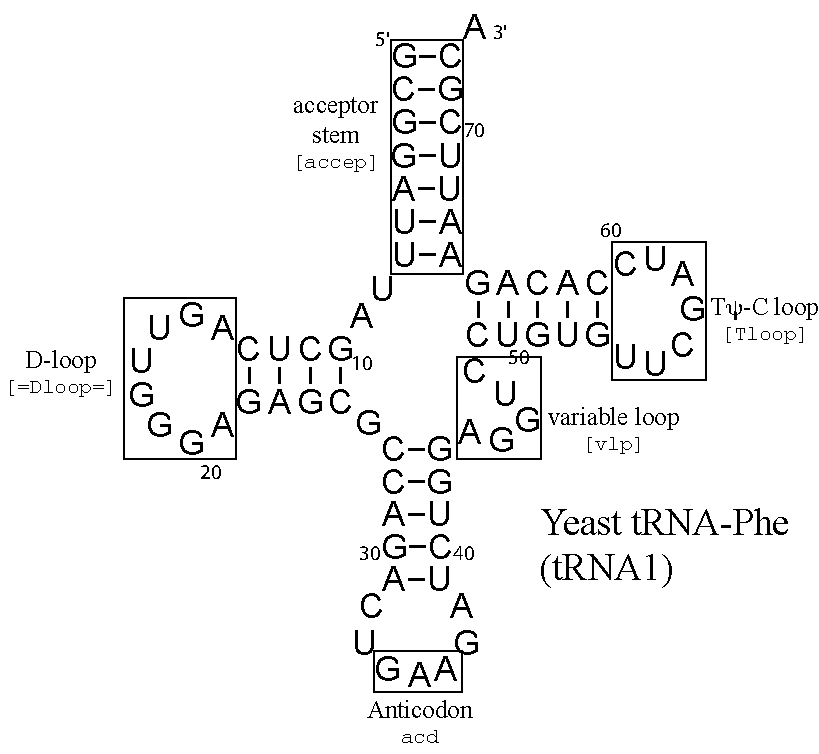
\includegraphics[scale=0.4]{Figures/trna1-DF6280-hand}
\end{minipage}
\vspace{1em}

This file is the same as \otext{tutorial/tRNA5.sto} except for the two
additional lines beginning with \otext{\#=GC RF}. This RF (reference)
annotation is required for using \otext{--hand}. Any non-gap character
in the reference annotation will be assigned as a match
position. Importantly, four different characters are considered gaps:
dashes (\otext{-}), underscores (\otext{\_}), dots (\otext{.}) and
tildes (\otext{~}). In this alignment, all columns are non-gap
characters, so all columns will be considered match positions.

Different regions of the secondary structure have been marked up using
abbreviations for the names of the regions in the reference
annotation. For example, \otext{acd} annotates the three positions of
the anticodon. I've used \otext{[} and \otext{]} to indicate region
boundaries in some cases. Crucially, I've avoided the use of any gap
characters for positions between named regions which I still want to
be considered match positions, and opted to use \otext{=} (which is
not considered a gap by \prog{cmbuild}) for these positions.

To build the hand-specified model from this alignment, do:

\user{cmbuild --hand tRNA5-hand.cm tutorial/tRNA5.hand.sto}

The output reports that the model now has 74 match (consensus)
positions in the \otext{clen} column. If we had built this model
without specifying \otext{--hand} (as we did earlier in this tutorial)
the resulting model would have had only 72 consensus positions.
(I've annotated the two extra match positions with three gaps in
\otext{tRNA5.hand.sto} as match solely to demonstrate how
\otext{--hand} works, not because I think it's better to model these
positions as matches than inserts.)

\begin{sreoutput}
# cmbuild :: covariance model construction from multiple sequence alignments
# INFERNAL 1.1 (June 2012)
# Copyright (C) 2012 Howard Hughes Medical Institute.
# Freely distributed under the GNU General Public License (GPLv3).
# - - - - - - - - - - - - - - - - - - - - - - - - - - - - - - - - - - - -
# CM file:                                            tRNA5-hand.cm
# alignment file:                                     ../tutorial/tRNA5-hand.sto
# use #=GC RF annotation to define consensus columns: yes
# - - - - - - - - - - - - - - - - - - - - - - - - - - - - - - - - - - - -
#                                                                      rel entropy
#                                                                      -----------
# idx    name                     nseq eff_nseq   alen  clen  bps bifs    CM   HMM description
# ------ -------------------- -------- -------- ------ ----- ---- ---- ----- ----- -----------
       1 tRNA5-hand                  5     3.59     74    74   21    2 0.763 0.476 
#
# CPU time: 0.36u 0.00s 00:00:00.36 Elapsed: 00:00:00.41
\end{sreoutput}

Now, let's use this model to search the \emph{M. ruminantium} genome
again. First, the model must be calibrated. To save time, a calibrated
version of the file is in \otext{tutorial/tRNA5-hand.c.cm}. To do the
search:

\user{cmsearch tutorial/tRNA5-hand.c.cm tutorial/mrum-genome.fa}

The results are very similar to the earlier search with the
tRNA model built with default \prog{cmbuild} parameters (though not
identical since the model now has two additional match positions). The
important difference involves the hit alignments. Take a look at the
alignment for hit number 46 as an illustrative example:

\begin{sreoutput}
>> NC_013790.1  Methanobrevibacter ruminantium M1 chromosome, complete genome
 rank     E-value  score  bias mdl mdl from   mdl to       seq from      seq to       acc trunc   gc
 ----   --------- ------ ----- --- -------- --------    ----------- -----------      ---- ----- ----
 (46) !   1.6e-09   43.2   0.0  cm        1       74 []      995344      995263 - .. 0.90    no 0.49
                                 v          v                                                            NC
                     (((((((,,<<<<________._>>>>,<<<<<_______>>>>>,,,........,,<<<<<_______>>>>>))))))): CS
   tRNA5-hand      1 gCcggcaUAGcgcAgUUGGuu.AgcgCgccagccUgucAagcuggAGg........UCCgggGUUCGAUUCcccGugccgGca 74    
                     :::G:CAUAGCG AG  GGU+ A CGCG:CAG:CU +++A:CUG: G+        UC:GGGGUUCGA UCCCC:UG:C:::A
  NC_013790.1 995344 AGAGACAUAGCGAAGC-GGUCaAACGCGGCAGACUCAAGAUCUGUUGAuuaguucuUCAGGGGUUCGAAUCCCCUUGUCUCUA 995263
                     ************9***.8886258***********************9444444445************************** PP
                     [accep]======[=Dloop=.]============acd=======[vl........p]=====[Tloop]=====[accep]= RF
\end{sreoutput}

The reference annotation from the training alignment to \prog{cmbuild}
has been propagated to the hit. All inserts in the alignment are
annotated as \otext{.} columns in the RF annotation. Note that the
variable loop (annotated as \otext{[vlp]} in the training alignment)
contains 8 inserted residues. The RF annotation will also be
transferred to multiple alignments created with \prog{cmalign}.

